\documentclass{article}

\usepackage[utf8]{inputenc} % For Unicode characters
\usepackage{amsmath}        % For mathematical symbols
\usepackage{graphicx}       % For including images
\usepackage{hyperref}       % For hyperlinks
\usepackage{geometry}      % For setting page margins
\usepackage{float}
\usepackage{tcolorbox}

% Set the page margins
\geometry{margin=1in}
% Set the top margins
\addtolength{\topmargin}{-.5in}

\title{Engineering Optics, Homework 2-Extra}
\author{He Tianyang}
\date{\today}

\begin{document}
\maketitle

\section{Problem 1}

1. An object 1cm high is 30cm in front of a thin lens with a focal length of 10cm. Where is the image? Verify your answer by graphical construction of the image.\\\\
\textbf{Solve:}\\

Given that $f' = 10cm$, $l = -30cm$. We can use the gaussian formula to find the image distance $l'$:
\begin{equation}
    \frac{1}{l'}-\frac{1}{l} = \frac{1}{f'}
\end{equation}

Therefore,
\begin{equation}
    l' = \frac{1}{\frac{1}{l} + \frac{1}{f'}} = \frac{1}{\frac{1}{-30} + \frac{1}{10}} = 15cm
\end{equation}

and the vertical magnification $\beta$ is
\begin{equation}
    \beta = \frac{l'}{l} = \frac{15}{-30} = -0.5
\end{equation}

So we have, the image height $h'$ is
\begin{equation}
    h' = \beta h = -0.5 \times 1 = -0.5cm
\end{equation}

To sum up, the image is $\mathbf{15cm}$ behind the lens,
and the image is $\mathbf{0.5cm}$ high.

Verify by graphical construction:
\begin{figure}[H]
    \centering
    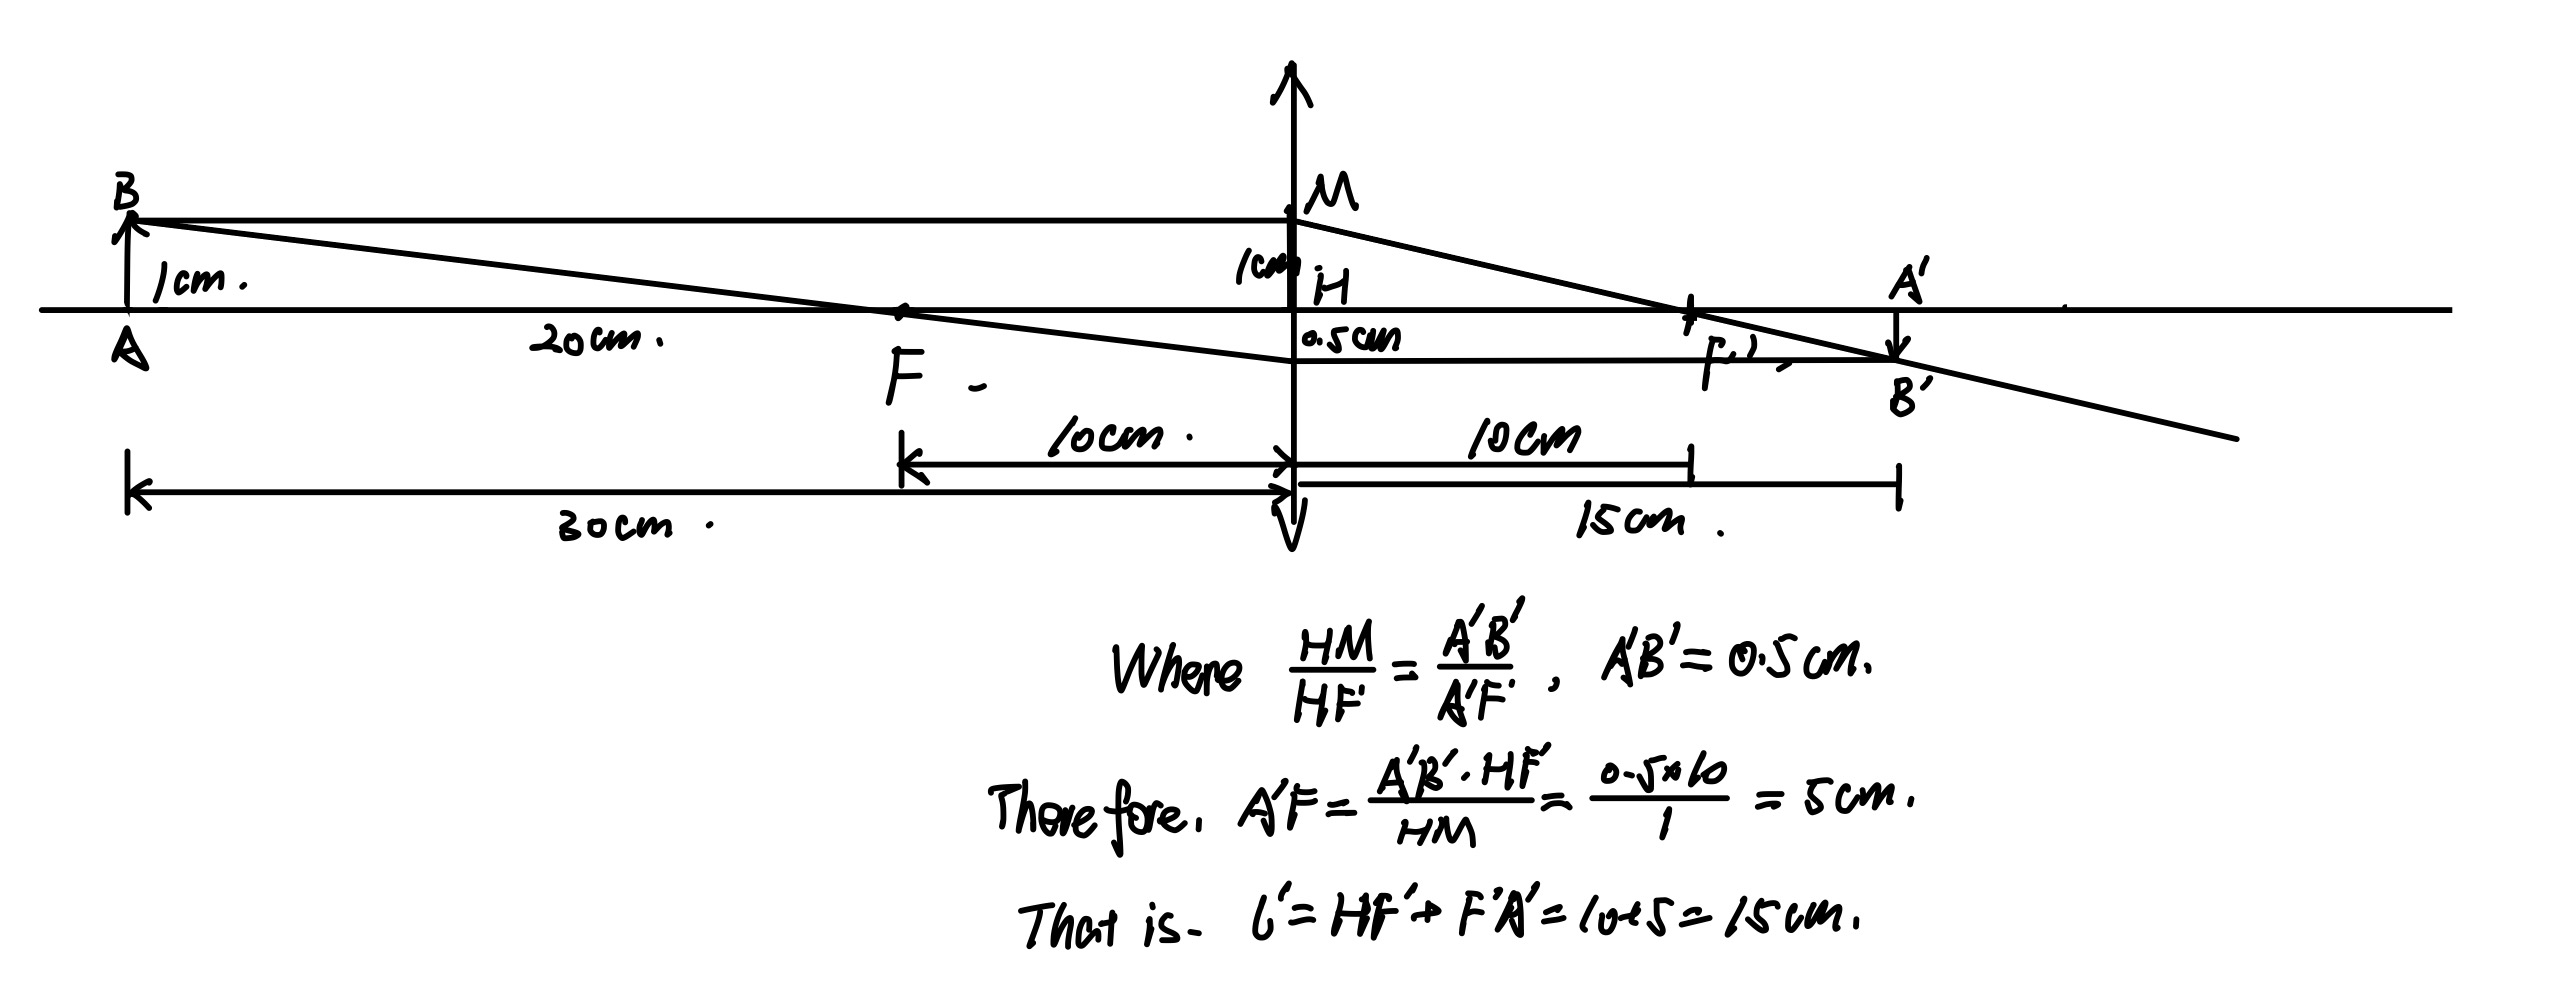
\includegraphics[width=0.9\textwidth]{./image/hw2/hw2e_1.jpeg}
    \caption{Graphical construction of the image}
\end{figure}

\textbf{The graphical construction is consistent with the calculation.}

\section{Problem 2}

2. A lens is known to have a focal length of 30cm in air. An object is placed 50cm to the left of the lens. Locate the image.\\\\
\textbf{Solve:}\\

Given that $f' = 30cm$, $l = -50cm$. We can use the gaussian formula to find the image distance $l'$:
\begin{equation}
    \frac{1}{l'}-\frac{1}{l} = \frac{1}{f'}
\end{equation}

Therefore,
\begin{equation}
    \boxed{
        l' = \frac{1}{\frac{1}{l} + \frac{1}{f'}} = \frac{1}{\frac{1}{-50} + \frac{1}{30}} = 75cm
    }
\end{equation}

and the vertical magnification $\beta$ is
\begin{equation}
    \beta = \frac{l'}{l} = \frac{75}{-50} = -1.5
\end{equation}

So we have, the image is $\mathbf{75cm}$ behind the lens, with a magnification of $\mathbf{-1.5}$.

\section{Problem 3}
3. A goldfish swims 10cm from the side of a spherical bowl of water of radius 20cm. Where does the fish appear to be?
Does it appear larger or smaller?\\\\
\textbf{Solve:}\\

The optical path is shown in the Figure \ref{fig:hw2e_3}.
\begin{figure}[H]
    \centering
    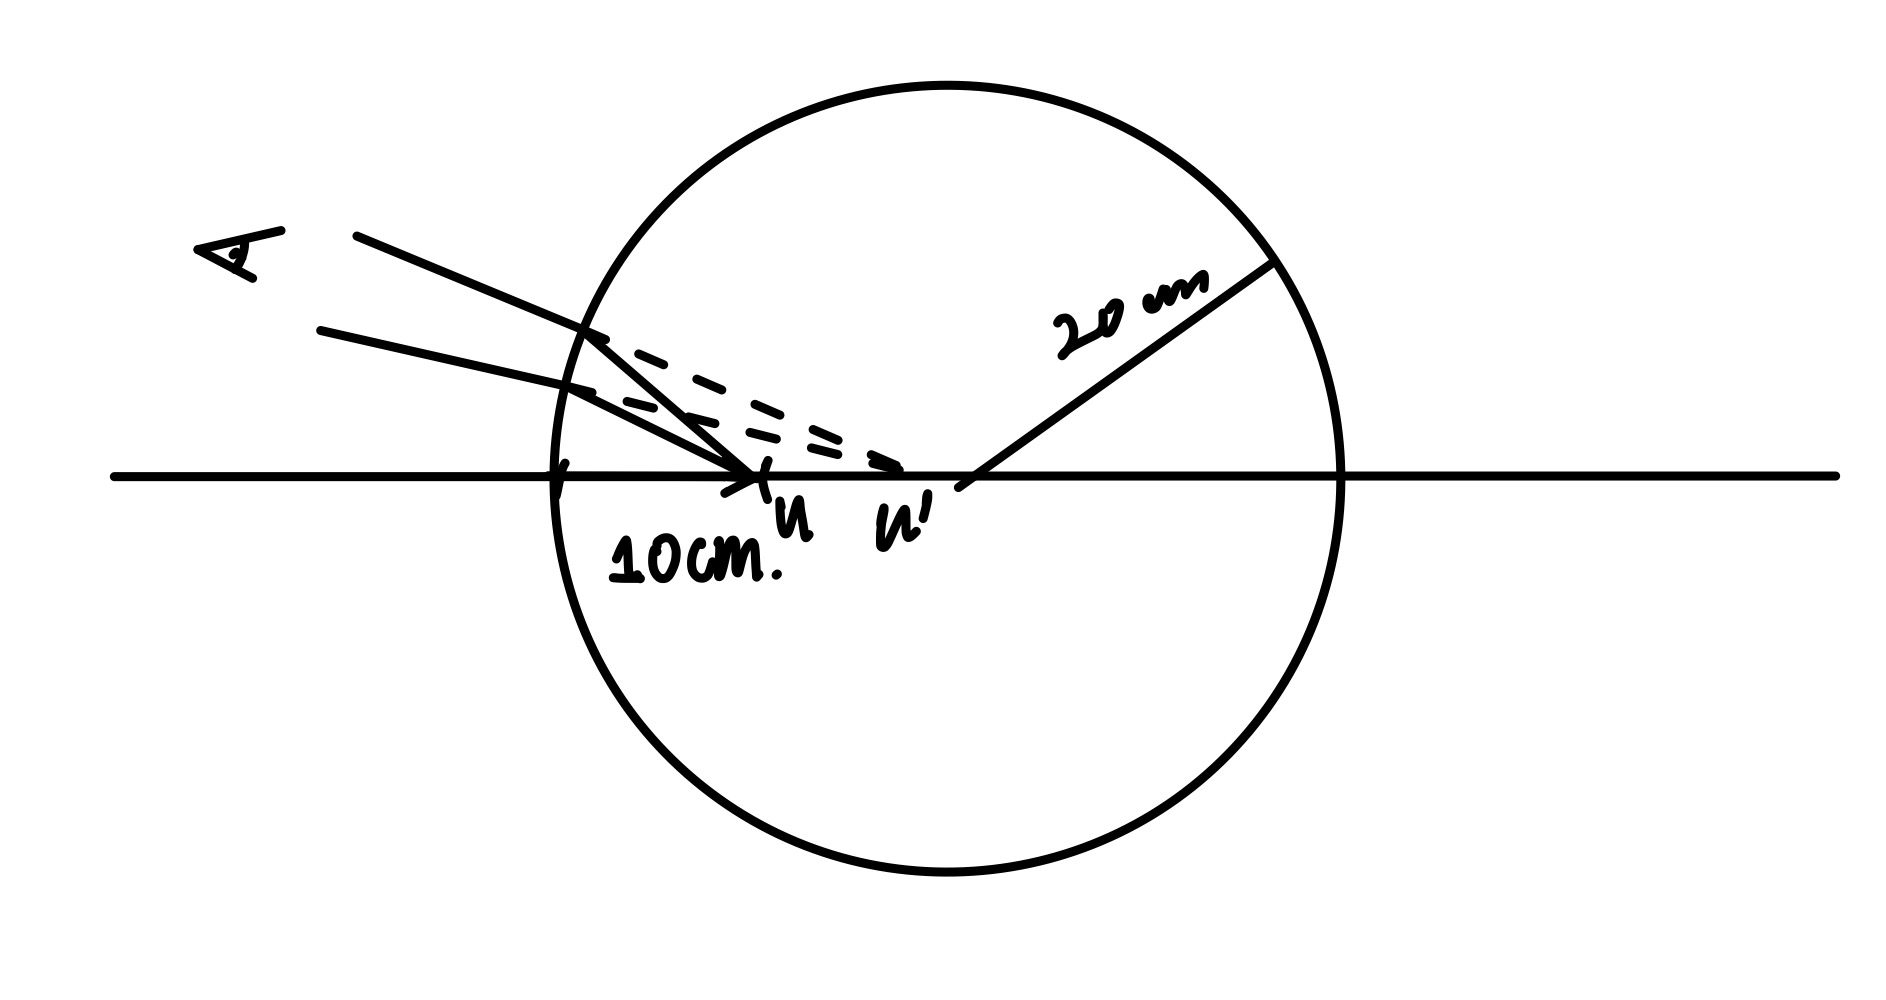
\includegraphics[width=0.5\textwidth]{./image/hw2/hw2e_3.jpeg}
    \caption{Optical path of the spherical bowl}
    \label{fig:hw2e_3}
\end{figure}

First, consider looks from the left side of the bowl, because the optical path is reversible, so given that $r = -20\mathbf{cm}$, $l = -10\mathbf{cm}$, $n \approx 1.33$, $n' = 1$. Therefore, we have:
\begin{equation}
    \frac{1}{l'} - \frac{1.33}{-10} = \frac{1-1.33}{-20}
\end{equation}

That is:
\begin{equation}
    \boxed{
        l' = \frac{20}{-2.33} \approx -8.58\mathbf{cm}
    }
\end{equation}

Where $l'$ is the distance from the left side of the bowl to the image.\\

to calculate the size of the image, we have:
\begin{equation}
    \boxed{
        \beta = \frac{nl'}{n'l} = \frac{1.33 \times (-8.58)}{1 \times (-10)} \approx 1.14
    }
\end{equation}

which means the image is $\mathbf{1.14}$ times the size of the fish, become \textbf{larger}.\\

Then, consider looks from the right side of the bowl, because the optical path is reversible, so given that $r = -\mathbf{20cm}$, $l = -30\mathbf{cm} $, $n = 1.33$, $n' = 1$. Therefore, we have:
\begin{equation}
    \frac{1}{l'} - \frac{1.33}{-30} = \frac{1-1.33}{-20}
\end{equation}

That is:
\begin{equation}
    \boxed{
        l' \approx -35.93\mathbf{cm}
    }
\end{equation}

Where $l'$ is the distance from the right side of the bowl to the image.

or we can format the variables using the left vertex as the origin, we have:
\begin{align}
    \boxed{
        l'' = d + l' = 40 - 35.93 = 4.07 \mathbf{cm}
    }
\end{align}

to calculate the size of the image, we have:
\begin{equation}
    \boxed{
        \beta = \frac{nl'}{n'l} = \frac{1.33 \times -8.58}{1 \times -30} \approx 0.38
    }
\end{equation}

which means the image is $\mathbf{0.38}$ times the size of the fish, become \textbf{smaller}.





\section{Problem 4}
4. An object is located 2cm to the left of convex end of a glass rod which has a radius of curvature of 1cm. The index of refraction of the glass is n=1.5. Find the image distance.\\\\
\textbf{Solve:}\\

Consider the glass rod as  a spherical lens, with the radius of curvature $r = 1cm$, and the object distance $l = -2cm$. The Optical path is shown in the Figure \ref{fig:hw2e_2}.
\begin{figure}[H]
    \centering
    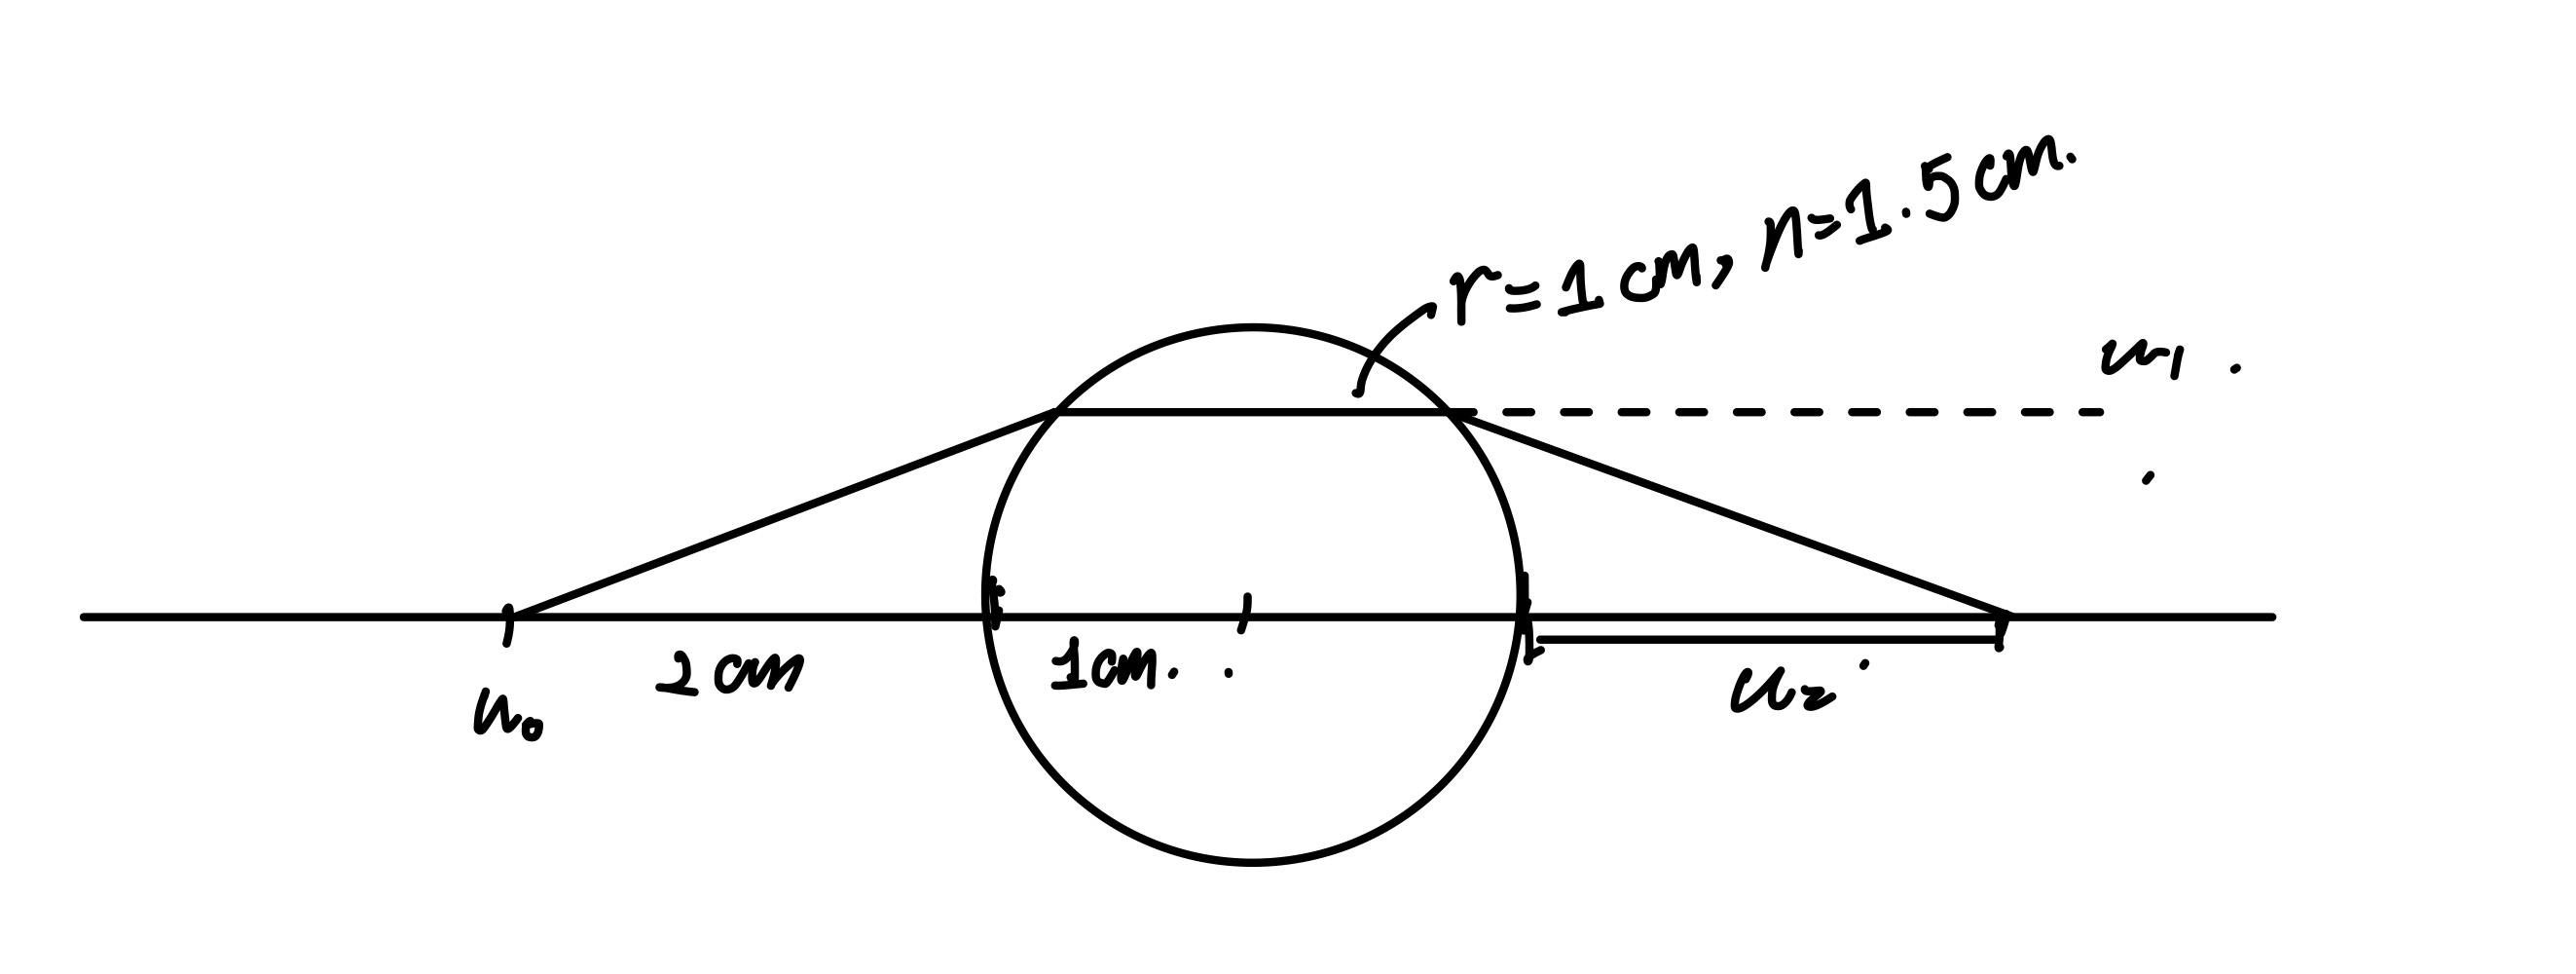
\includegraphics[width=0.6\textwidth]{./image/hw2/hw2e_2.jpeg}
    \caption{Optical path of the glass rod}
    \label{fig:hw2e_2}
\end{figure}

And assuming this is the adaxial situation, the image follows:
\begin{equation}
    \frac{n'}{l'} - \frac{n}{l} = \frac{n'-n}{r}
\end{equation}

First, consider the left surface of the glass rod, we have:
\begin{equation}
    \frac{1.5}{u_1} - \frac{1}{-2} = \frac{1.5-1}{1}
\end{equation}

Solving this equation, we have:
\begin{equation}
    \boxed{
        u_1 = \infty
    }
\end{equation}

That means the optical path is parallel to the optical axis after the left surface of the glass rod.\\

Then, consider the right surface of the glass rod, we should transform the variables using the right vertex as the origin. we have:
\begin{align}
     & l =  - \infty      \\
     & r =  -1\mathbf{cm} \\
     & n =  1.5           \\
     & n'=  1             \\
\end{align}

Therefore, we have:
\begin{equation}
    \frac{1}{l'} - \frac{1.5}{-\infty} = \frac{1-1.5}{-1}
\end{equation}

Solving this equation, we have:
\begin{equation}
    \boxed{
        l' =2\mathbf{cm}
    }
\end{equation}

Where $l'$ is the distance from the right vertex of the rod to the image.

\section{Problem 5}

5. The object is a transparent cube, 4mm across, placed 60cm in front of a lens of 20cm focal length.
Calculate the transverse and axial magnification and describe what the image looks like?\\\\
\textbf{Solve:}\\

Given that $f' = 20\mathbf{cm}$, $l = -60\mathbf{cm}$, $y = 4\mathbf{mm}$, $n = 1$, $n' = 1$. We can use the gaussian formula to find the image distance $l'$:

\begin{equation}
    \frac{1}{l'}-\frac{1}{-60} = \frac{1}{20}
\end{equation}

Therefore,
\begin{equation}
    \boxed{
        l' = \frac{1}{\frac{1}{-60} + \frac{1}{20}} = 30\mathbf{cm}
    }
\end{equation}

Calculating the vertical magnification and the axial magnification $\beta$ and $\alpha'$:
\begin{equation}
    \boxed{
        \begin{aligned}
            \beta  & = \frac{l'}{l} = \frac{30}{-60} = -0.5 \\
            \alpha & =  \beta^2 = 0.25
        \end{aligned}
    }
\end{equation}

That means, the image is $\mathbf{30cm}$ behind the lens, with width $\mathbf{1mm}$ and height $\mathbf{2mm}$. The image become a cuboid, with the width and height ratio of 1:2, and the image is \textbf{inverted} on the vertical.


\end{document}